\section{Skalieren von Bildern}
\label{scale_Algos}
Da die Berechnungen meist auf recht kleinen Bildausschnitten ausgeführt wird, müssen diese für weitere Rechenschritte hochskaliert werden, damit es von OpenFace besser verarbeitet wird.\\
Dabei ist es wichtig, dass die Gesichtsmerkmale möglichst gut rekonstruiert werden, um die entsprechenden Landmarks zu bestimmen. Dazu können verschiedene Verfahren verwendet werden.
\subsection{Nearest-Neighbor-Skalierung}
Dieses Verfahren verwendet als neuer Farbwert, den gleichen Wert wie das nächstgelegene Pixel. Dadurch werden nur die ehemaligen Pixel größer und das Gesicht wirkt sehr Kantig, da keine neuen Farbwerte bestimmt werden, siehe \autoref{img_NN}. Bei der Vergrößerung des Schachbretts ist kein Fehler aufgetreten, da nur zwei Farben vorhanden und Positionsabhängig sind.
\subsection{Linear-Skalierung}
Um den neuen Farbwert zu ermitteln, wird zwischen den nächst gelegenen umliegenden Pixel linear Interpoliert, wodurch weitere Farbwerte entstehen. Das Ergebnis ist gleichmäßiger als Neares Neighbor, und dennoch ein recht einfaches Verfahren. Die Kanten wirken allerdings unscharf, siehe \autoref{img_Linear}.
\subsection{Bicubic-Skalierung}
Um den Farbwert zu ermitteln, werden die umliegenden $4\times 4$ Pixelwerte betrachtet um den Farbverlauf als eine Funktion 3. Grades zu bestimmen. Somit werden feinere Details besser dargestellt als beim linearen Verfahren und Kanten bleiben eher erhalten. Allerdings kann es durch den bestimmten Verlauf auch zum Überschwingen kommen, wodurch Fehlfarben entstehen können. Ein Beispiel ist in \autoref{img_Bicubic} zu sehen.
\cite{wiki_Bicubic}
\subsection{Lanczos-Skalierung}
Dieser Filter basiert auf einem bewerteten Durchschnitt er umliegenden Pixel. Die Bewertung der einzelnen Pixel wird mit einer Sinc-Funktion bestimmt damit weiter entferntere Pixel schwächer zu bewerten als die nächstliegenden, um den neuen Pixelwert zu erhalten.\\
Außerdem wird durch den Kurvenverlauf der Bewertungsfunktion eine gewisse Bildschärfe erreicht, siehe \autoref{img_Lanczos}. Die Funktion kann und wird für die Anwendung auf einen $8\times 8$ Pixel großen Bereich begrenzt. \cite{wiki_Lanczos}
\[ L(x)= \left\{ \begin{array}{ll}
\frac{\sin(\pi x)}{\pi x} \cdot \frac{\sin(\pi \frac{x}{a})}{\pi \frac{x}{a}} & \textrm{wenn } -a < x <a, a\neg 0\\
1 & \textrm{wenn } x = 0\\
0 & \textrm{sonst}
\end{array}\right. \]
\begin{figure}
	\centering
	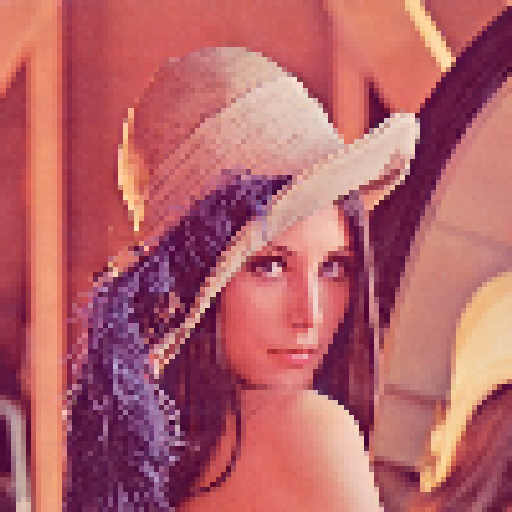
\includegraphics[width=0.2\linewidth]{img/lena100_NN}
	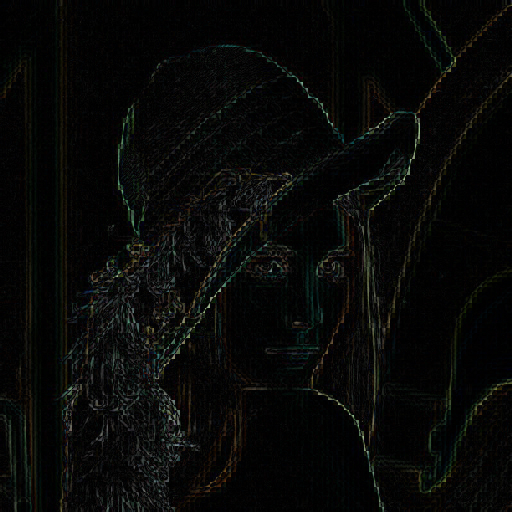
\includegraphics[width=0.2\linewidth]{img/lena100_NN_differenz}
	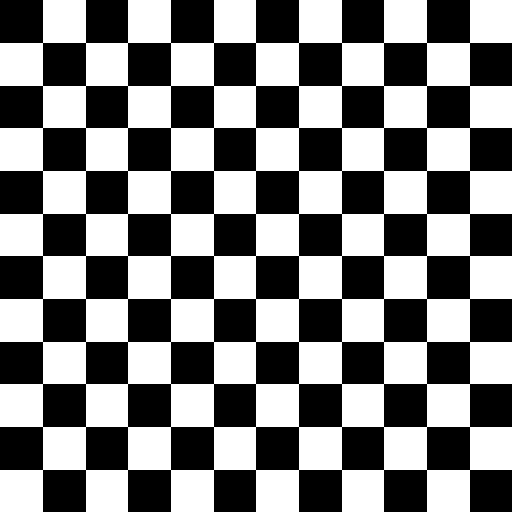
\includegraphics[width=0.2\linewidth]{img/Schachbrett_NN}
	\caption{Die ursprüngliche Abbildung von Lena betrug 100 Pixel Kantenlänge und beim Schachbrett 48 Pixel, beide wurden mittels Nearest-Neighbor auf 512 Pixel vergrößert und bei Lena die Differenz zum originalen Lena-Bild bestimmt}
	\label{img_NN}
\end{figure}
\begin{figure}
	\centering
	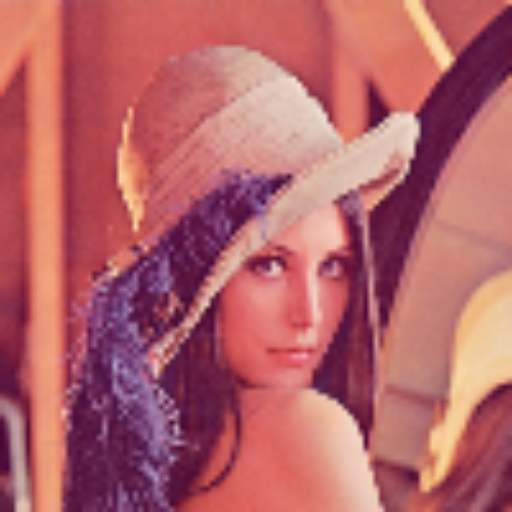
\includegraphics[width=0.2\linewidth]{img/lena100_LINEAR}
	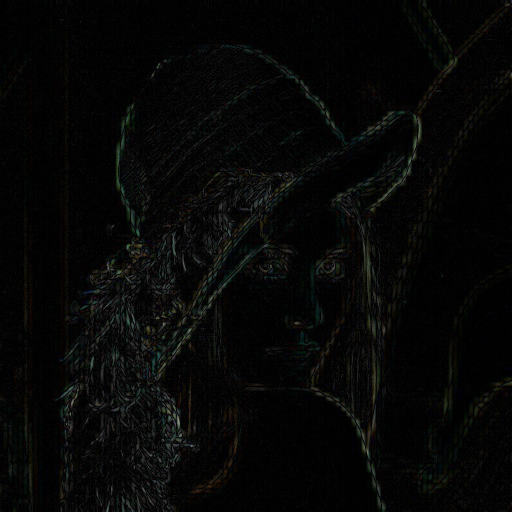
\includegraphics[width=0.2\linewidth]{img/lena100_LINEAR_differenz}
	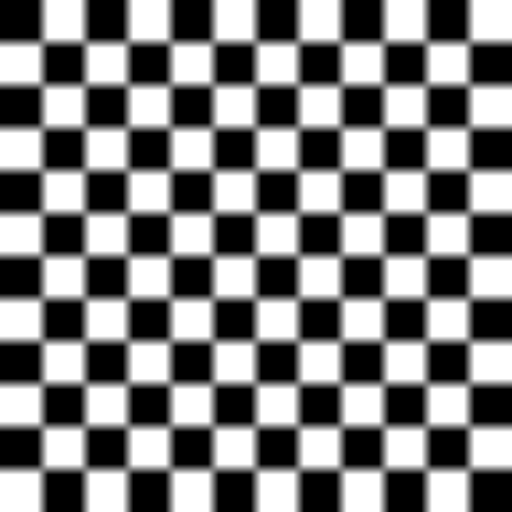
\includegraphics[width=0.2\linewidth]{img/Schachbrett_LINEAR}
	\caption{Die ursprüngliche Abbildung von Lena betrug 100 Pixel Kantenlänge und beim Schachbrett 48 Pixel, beide wurden mittels linearer Interpolation auf 512 Pixel vergrößert und bei Lena die Differenz zum originalen Lena-Bild bestimmt}
	\label{img_Linear}
\end{figure}
\begin{figure}
	\centering
	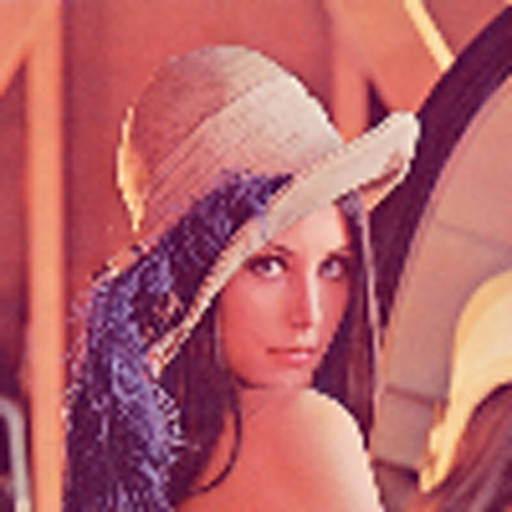
\includegraphics[width=0.2\linewidth]{img/lena100_CUBIC}
	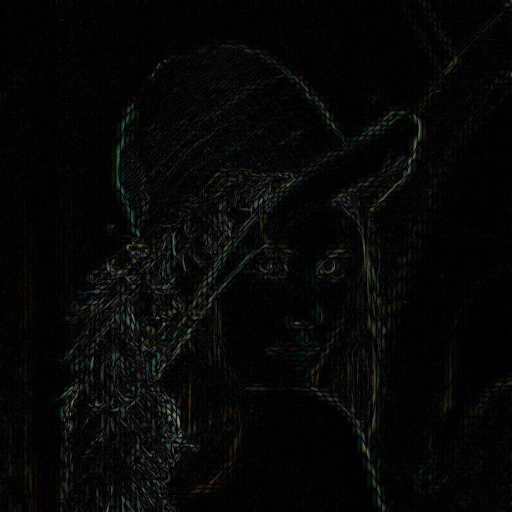
\includegraphics[width=0.2\linewidth]{img/lena100_CUBIC_differenz}
	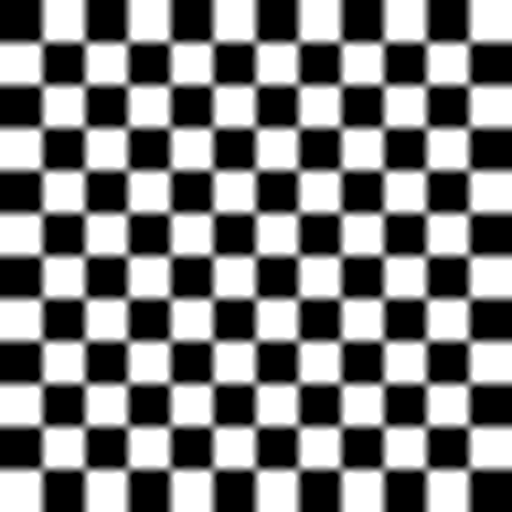
\includegraphics[width=0.2\linewidth]{img/Schachbrett_CUBIC}
	\caption{Die ursprüngliche Abbildung von Lena betrug 100 Pixel Kantenlänge und beim Schachbrett 48 Pixel, beide wurden mittels bikubischem Verfahren auf 512 Pixel vergrößert und bei Lena die Differenz zum originalen Lena-Bild bestimmt}
	\label{img_Bicubic}
\end{figure}
\begin{figure}
	\centering
	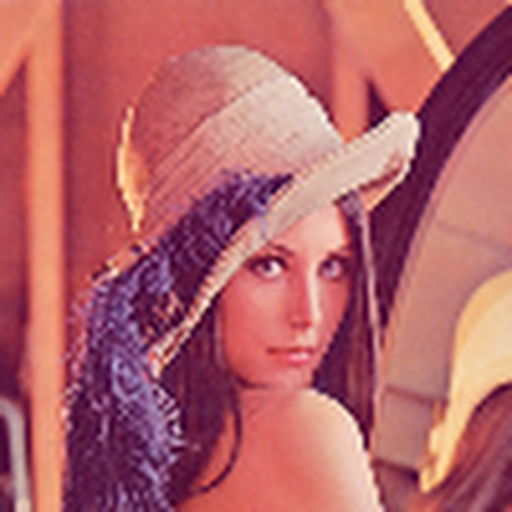
\includegraphics[width=0.2\linewidth]{img/lena100_LANCZOS4}
	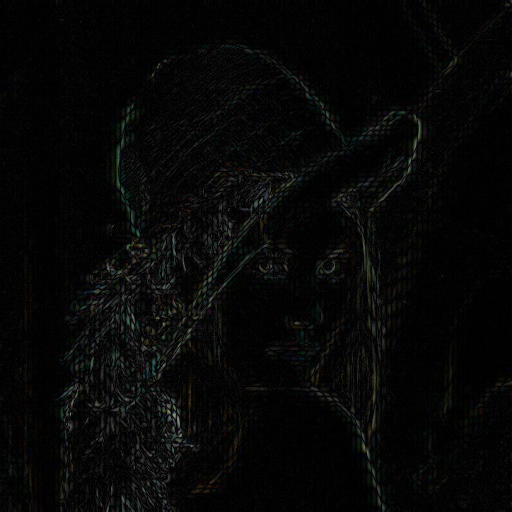
\includegraphics[width=0.2\linewidth]{img/lena100_LANCZOS4_differenz}
	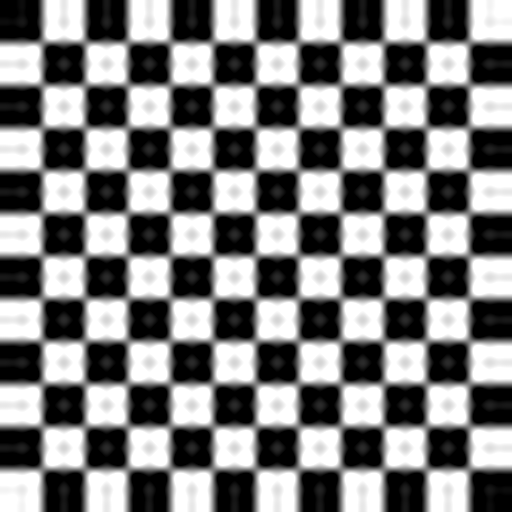
\includegraphics[width=0.2\linewidth]{img/Schachbrett_LANCZOS4}
	\caption{Die ursprüngliche Abbildung von Lena betrug 100 Pixel Kantenlänge und beim Schachbrett 48 Pixel, beide wurden mittels Lanczus-Verfahren auf 512 Pixel vergrößert und bei Lena die Differenz  zum originalen Lena-Bild bestimmt}
	\label{img_Lanczos}
\end{figure}
%% http://docs.opencv.org/2.4/modules/imgproc/doc/geometric_transformations.html#resize